\section{作成した教材}

\subsection{動的計画法とは}
\noindent
{\LARGE そもそもアルゴリズムって?}\\ \hrulefill \\
アルゴリズムとは、何かの処理を行う際の手順を表すものです。
これはよく料理のレシピに例えられます。

\noindent
料理をする時、多くの人はレシピを参考にします。
料理のレシピには材料や分量、調理の手順などが載っていて、料理をするときにはそのレシピの通りに調理をしてやれば美味しい料理を作ることができます。
材料や分量が同じでも、調味料や手順を間違えると、カレーを作ろうとしたのに肉じゃがになったりシチューになったり、はたまた食べられないダークマターのようなものになったりしてしまいます。\\
\noindent
プログラミングではこの材料や分量にあたる部分がデータ、調理の手順がアルゴリズムと呼ばれています。 
\\ \\
\noindent
{\LARGE アルゴリズムを知る、ということ}\\ \hrulefill \\
僕たちは普段から様々な料理と親しんでいるので美味しい食べ方のできるレシピを何となくでイメージすることも調べることもできます。
たとえば「魚を食べたい!」と思ったら、刺身、湯がく、茹でる、煮る、焼く、揚げる、蒸す、燻す…と色々な調理法が思い浮かびます。

\noindent
アルゴリズムの場合も同じように、様々なアルゴリズムを「知って」いれば何となく使えそうなアルゴリズムをイメージしたり調べたりすることができるようになります。

\noindent
本教材では\emph{動的計画法}というアルゴリズムのみを扱いますが、もし興味があれば是非色々なアルゴリズムを「知って」「使って」みてください。 
\\ \\
\noindent
{\LARGE 動的計画法とは}\\ \hrulefill \\
動的計画法(Dynamic Programming : 以下DP)は、求めたい問題を複数の部分問題に分け、部分問題を計算・記録しながら解いていくことにより元の問題の答えを導く手法のことです。

\noindent
…と言ってもイマイチ分かりづらいので、本教材でのDPは

\noindent
①(部分問題に)\emph{分ける}\\
②(計算結果を)\emph{メモる}\\
③(メモを元に)\emph{求める}

\noindent
の3ステップで考えていきたいと思います。\\

\clearpage

\subsection{動的計画法の考え方}
\subsubsection{導入 例題(線形探索問題)の紹介}

\noindent
まずは動的計画法の3ステップ

\noindent
①\emph{分ける}\\
②\emph{メモる}\\
③\emph{求める}

\noindent
について見ていきます。 
\\ \\
\noindent
この章では次の問題について考えます。\\
\hrulefill \\
\emph{例題1} \\
長さ $N$ の整数列 $A=$ \{$A_0,A_1,...,A_{N-1}$\} が与えられます。

\noindent
$A$ に含まれる最大の数を求めなさい。

\noindent
・$1 \leq N \leq 10^5$

\noindent
・$-10^6 \leq A_i \leq 10^6$

\noindent
入力

\noindent
$N$

\noindent
$A_0 A_1 ... A_{N-1}$\\
\hrulefill \\
いわゆる線形探索法と呼ばれる問題です。

\noindent
一応、以下に線形探索における解答コードを載せておきます。

\noindent
読むとヒントになるかもしれませんが、別に読まなくても大丈夫です。

\clearpage
\noindent
\begin{lstlisting}[style = customC]
#include <stdio.h>

int main(void)
{
    /* n:要素数 a:入力される整数列 */
    int n, a[100000];
    /* res:答えを格納する変数 */
    /* 最大値を求める問題なので初期値を十分に小さい数にする */
    int res = - 2 << 30;

    /* 入力 */
    scanf("%d", &n);

    for(int i = 0; i < n; i++){
        scanf("%d", &a[i]);
    }
    /* 入力ここまで */

    /* aの各要素とresを比較し、a[i]の方が大きい場合resを更新する */
    for(int i = 0; i < n; i++){
        if(res < a[i]){
            res = a[i];
        }
    }

    printf("%d", res);

    return 0;
}
\end{lstlisting}

\noindent
線形探索による解法では、求める数に対して十分に小さい値を初期値とし、配列の全ての要素と順番に比較していくことにより求められます。
\\ \\
\noindent
今回はこの問題をDPの考え方をもとに解いていきます。

\clearpage

\subsubsection{部分問題に分ける}
\hrulefill \\
\emph{例題1} \\
長さ $N$ の整数列 $A=$ \{$A_0,A_1,...,A_{N-1}$\} が与えられます。

\noindent
$A$ に含まれる最大の数を求めなさい。

\noindent
・$1 \leq N \leq 10^5$

\noindent
・$-10^6 \leq A_i \leq 10^6$

\noindent
入力

\noindent
$N$

\noindent
$A_0 A_1 ... A_{N-1}$\\
\hrulefill \\

\noindent
まずは最初のステップとして、①分けるについて考えます。

\noindent
今回の問題の場合、複数の数字を比較して最大のものを選ぶ必要があります。

\noindent
僕たちの場合は適当に数字が並んでたらその中から一番大きいものを何となくで選べますが、プログラムでは2つのものしか比較ができません。

\noindent
そこで、この問題を以下のような部分問題に分割してみます。

\begin{itemize}
    \item $A_0$と$A_1$のうち大きいものを求める
    \item $A_1$までの最大値と$A_2$のうち大きいものを求める
    \item $A_2$までの最大値と$A_3$のうち大きいものを求める \\:
    \item $A_{N-2}$までの最大値と$A_{N-1}$のうち大きいものを求める
\end{itemize}

\noindent
実は、これをそのまま実装すると線形探索のコードと同じものが出来上がるんですけど今回はもうちょっと工程を増やします。

\noindent
次の節では②メモるについて見ていきますが、まずはC言語の文法の復習がてら次の練習問題を解いてみてください。

\clearpage

\subsubsection{2数の比較}
\noindent
{\LARGE 問題文}\\ \hrulefill \\

\noindent
整数 $X, Y$ が与えられます。

\noindent
2つの整数のうち、大きいほうの整数を答えてください。
\\ \\
\noindent
{\LARGE 制約}\\ \hrulefill \\

\noindent
・-100 $\leq X,Y \leq$ 100

\noindent
・$X \neq Y$
\\ \\
\noindent
{\LARGE 入力}\\ \hrulefill \\

\noindent
入力は以下の形式で標準入力から与えられる。 

\noindent
$X Y$
\\ \\
\noindent
{\LARGE 出力}\\ \hrulefill \\

\noindent
1行で、大きいほうの整数を出力せよ。

\clearpage

\subsubsection{問題の解説}
\noindent
プログラムで2つの値を比較する場合にはif文による分岐が利用できます。\\
よって、以下のいずれかの方針で実装することができます。

\begin{itemize}
    \item $X$の方が大きければ$X$を、それ以外の場合は$Y$を出力する
    \item $X$の方が小さければ$Y$を、それ以外の場合は$X$を出力する
    \item $Y$の方が大きければ$Y$を、それ以外の場合は$X$を出力する
    \item $Y$の方が小さければ$X$を、それ以外の場合は$Y$を出力する
\end{itemize}

\noindent
解答例は以下のようになります。

\noindent
\begin{lstlisting}[style = customC]
#include <stdio.h>

int main(void)
{
    /* 入力 */
    int x, y;
    scanf("%d %d", &x, &y);

    if(x > y){
        printf("%d", x);
    }else{
        printf("%d", y);
    }

    return 0;
}
\end{lstlisting}

\noindent
また、max()などの最大値を返す関数を別に実装するとmain関数内での記述がわかりやすくなります。

\noindent
\begin{lstlisting}[style = customC]
#include <stdio.h>

int max(int x, int y) {
        return x > y ? x : y; 
}

int main(void) {
    /* 入力 */
    int x, y;
    scanf("%d %d", &x, &y);

    printf("%d", max(x, y));

    return 0;
}
\end{lstlisting}

\noindent
Java/Python/C++の解答例は以下を確認してください。\\
解答例(Gist)[リンク]

\clearpage

\subsubsection{Gistの解答例}
\noindent
基本的にすべての言語にmax関数が用意されているためそれを利用することができます。\\
max関数を利用しない場合はC言語と同様の実装をしてください。
\\ \\
\noindent
C++による解答例
\begin{lstlisting}[style = customCpp]
// C++の場合
// 実行環境ではbits/stdc++.hのインクルードが可能ですが、
// VisualC++等の環境で開発を行っている場合は手元でコンパイルできない可能性があるため
// ヘッダファイルをそれぞれインクルードしてください

#include <bits/stdc++.h>
// #include <algorithm>
// #include <iostream>

using namespace std;

int main(void) { 
    int x, y;
    cin >> x >> y;

    cout << max(x, y) << endl;
    
    return 0;
}
\end{lstlisting}

\noindent
Javaによる解答例
\begin{lstlisting}[style = customJava]
// Javaの場合
// クラス名をMainとする必要があります

import java.util.*;

public class Main{
    public static void main(String[] args) {
        int x, y;
        Scanner sc = new Scanner(System.in);
        x = Integer.parseInt(sc.next());
        y = Integer.parseInt(sc.next());

        System.out.println(Math.max(x, y));
    }
}
\end{lstlisting}

\noindent
Python3による解答例
\begin{lstlisting}[style = customPy]
# Pythonの場合
# x if x > y else y等の記述でも可能です

x, y = map(int, input().split())

print(max(x, y))
\end{lstlisting}

\clearpage

\subsubsection{計算結果をメモする}
\hrulefill \\
\emph{例題1} \\
長さ $N$ の整数列 $A=$ \{$A_0,A_1,...,A_{N-1}$\} が与えられます。

\noindent
$A$ に含まれる最大の数を求めなさい。

\noindent
・$1 \leq N \leq 10^5$

\noindent
・$-10^6 \leq A_i \leq 10^6$

\noindent
入力

\noindent
$N$

\noindent
$A_0 A_1 ... A_{N-1}$\\
\hrulefill \\
\noindent
①分けるにより、今回の問題は以下のような部分問題にすることが出来ました。

\begin{itemize}
    \item $A_0$と$A_1$のうち大きいものを求める
    \item $A_1$までの最大値と$A_2$のうち大きいものを求める
    \item $A_2$までの最大値と$A_3$のうち大きいものを求める \\:
    \item $A_{N-2}$までの最大値と$A_{N-1}$のうち大きいものを求める
\end{itemize}
\noindent
次のステップとして、②メモるについて考えていきます。
\\ \\
\noindent
そもそも、ここで言うメモとは何か?という話なんですが、これは「計算結果を記録しておく」ことを表しています。 \\ 
普段の生活でするメモと同じように、とりあえず忘れないように残しとこ~って感じの使い方ですね。
\\ \\
\noindent
じゃあDPでは何をメモするのか、というと「部分問題を解いた時に出てきた解」をメモしておきます。\\
今回の場合は$A_1$までの最大値、$A_2$までの最大値、…がメモに残る感じですね。
\\ \\ \noindent
部分問題を解きながらメモをしていくと、大体の場合は元の問題の答えが勝手に求められます。\\
今回の場合は$A_{N-1}$までの最大値がそのまま答えになっています。
\\ \\ \noindent
そのため、③求めるパートでは答えを出力するだけになることが多いです。\\
\clearpage
\noindent
次に、メモの方法について説明します。\\
といっても慣例的なものなのでこれじゃなきゃダメ!といったものではないのですが、色々なコード等を読む上で使ってる人が多い方法なので今回はこの方法を使ってみてください。
\\ \\ \noindent
メモを残すときには基本的には配列を利用します。\\
配列名は慣例的にdp、もしくはDPが利用されることが多いです。(memoやMEMOなどを使う人もいます)

\begin{lstlisting}[style = customC]
/* どちらでもいい */
int dp[100];
int DP[100];
\end{lstlisting}

配列の要素数は人により考え方が異なりますが
\begin{lstlisting}[style = customJava]
/* 要素数Nの上限が決まっている場合 */
int n_max = 100;

/* ①必要数ピッタリで作る */
int dp[100];

/* ②必要数より少し多めに作る */
int dp[110];
\end{lstlisting}

といった手法を取ることが多いです。
\\ \\ \noindent
それぞれのメリットとしては\\
①…メモリ使用量が減る\\
②…配列参照のエラーが起こりづらくなる\\
といった点があります。
\\ \\ \noindent
どちらを使っても問題ないのですが、C言語の場合①のメリットが非常に薄いので②を使うのがいいかな、と思います。\\
他言語を使う場合は①にも大きなメリットがある場合があるので好みによって使い分けてください。
\\ \\ \noindent
以上の内容を元に、次の節では具体例を見ていきます。

\clearpage

\subsubsection{問題を解く}
\hrulefill \\
\emph{例題1} \\
長さ $N$ の整数列 $A=$ \{$A_0,A_1,...,A_{N-1}$\} が与えられます。

\noindent
$A$ に含まれる最大の数を求めなさい。

\noindent
・$1 \leq N \leq 10^5$

\noindent
・$-10^6 \leq A_i \leq 10^6$

\noindent
入力

\noindent
$N$

\noindent
$A_0 A_1 ... A_{N-1}$\\
\hrulefill \\

\noindent
①分けるにより、今回の問題は以下のような部分問題にすることが出来ました。

\begin{itemize}
    \item $A_0$と$A_1$のうち大きいものを求める
    \item $A_1$までの最大値と$A_2$のうち大きいものを求める
    \item $A_2$までの最大値と$A_3$のうち大きいものを求める \\:
    \item $A_{N-2}$までの最大値と$A_{N-1}$のうち大きいものを求める
\end{itemize}
\noindent
また、dp配列を用いたメモを使うといい、という話がありました。
\\ \\ \noindent
ここからは具体的な例を元に解き方を考えていきます。
\\ \\ \noindent
例として、
$N=5$, $A=$\{$5,-3,2,9,-8$\}
というサンプルについて考えてみます。
\\ \\ \noindent
これに対してdp配列を用意するのですが、ちょっと工夫してこんな形にしてみます。

\begin{itemize}
    \item $dp[i](0 \leq i < N)$は$A[i]$までの最大値
\end{itemize}

\noindent
つまり、①分けるで考えたパターンに加えて、$dp[0]$は$A[0]$までの最大値、というイメージを追加している感じです。
\\ \\ \noindent
このようにすると、以下の図のように配列dpと配列Aの添字を揃えて考えることができるようになるので管理がしやすくなります。

\begin{figure}[H]
    \centering
    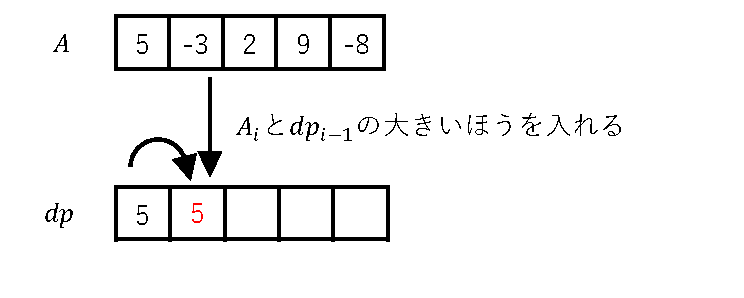
\includegraphics[width=0.7\linewidth, clip]{1-4.pdf}
\end{figure}

\noindent
実はdpなんていらないのは最初に説明しちゃったんですが、折角なのでこれらの内容を利用して、例題を「dp配列を利用して」解いてみてください。

\clearpage

\subsubsection{数列内の最大の数の出力}
\noindent
{\LARGE 問題文}\\ \hrulefill \\

\noindent
長さ $N$ の整数列 $A=$ \{$A_0,A_1,...,A_{N-1}$\} が与えられます。

\noindent
$A$ に含まれる最大の数を求めなさい。
\\ \\
\noindent
{\LARGE 制約}\\ \hrulefill \\

\noindent
・$2 \leq N \leq 10^5$

\noindent
・$-10^6 \leq A_i \leq 10^6$
\\ \\
\noindent
{\LARGE 入力}\\ \hrulefill \\

\noindent
入力は以下の形式で標準入力から与えられる。 

\noindent
$N$ \\
$A_1 A_2 ... A_N$
\\ \\
\noindent
{\LARGE 出力}\\ \hrulefill \\

\noindent
1行で、$A$ に含まれる最大の数を出力せよ。

\clearpage

\subsubsection{問題の解説}

\noindent
基本的には途中計算をメモしておくための配列(今回はdp)を用意したうえで、

\begin{itemize}
    \item $dp[i](0 \leq i < N)$は$A[i]$までの最大値
\end{itemize}

\noindent
という式をそのまま実装する形になります。
\\ \\ \noindent
今回$i$の値は0から$N-1$まで増加していくため、for文を利用してループしてやれば$dp[0]$から順に計算していくことができます。
\\ \\ \noindent
注意点として、$dp[-1]$は配列の添字として利用できないため、$i=0$の時のみ処理を分けるか$dp[0]=A[0]$という形にして$i=1$からループを開始するとよいです。
\\ \\ \noindent
以下に解答例を示します。

\noindent
\begin{lstlisting}[style = customC]
#include <stdio.h>

int main() 
{
    int n, a[100000], dp[100000];

    /* 入力 */
    scanf("%d", &n);
    for (int i = 0; i < n; i++) {
        scanf("%d", &a[i]);
    }

    dp[0] = a[0];

    for (int i = 1; i < n; i++) {
        if (a[i] > dp[i - 1]) {
            dp[i] = a[i];
        } else {
            dp[i] = dp[i - 1];
        }
    }

    printf("%d", dp[n - 1]);

    return 0;
}
\end{lstlisting}

\clearpage
\noindent
また、大きい数と同様にmax()関数などの大きいほうの数を返す関数を実装すると分かりやすくなります。\\
以下に解答例を示します。

\noindent
\begin{lstlisting}[style = customC]
#include <stdio.h>

int max(int x, int y) 
{ 
    return x > y ? x : y; 
}

int main()
{
    /* 入力 */
    int n, a[100000], dp[100000];
    scanf("%d", &n);

    for (int i = 0; i < n; i++) {
        scanf("%d", &a[i]);
    }

    dp[0] = a[0];

    for (int i = 1; i < n; i++) {
        dp[i] = max(dp[i - 1], a[i]);
    }

    printf("%d", dp[n - 1]);

    return 0;
}
\end{lstlisting}

\noindent
Java/Python/C++の解答例は以下を確認してください。\\
解答例(Gist)[リンク]

\clearpage

\subsubsection{Gistの解答例}
\noindent
基本的にはC言語と同様の実装が可能です。
\\ \\ \noindent
なお、C++のmax\_element関数、Pythonのmax()関数などを使うと配列内の最大値を求めることもできます。 今回は一応DPを使おう!という問題なので解答例はDPを利用した解答を示します。
\\ \\
\noindent
C++による解答例
\begin{lstlisting}[style = customCpp]
#include <bits/stdc++.h>
// #include <iostream>

using namespace std;

int main(void) {
    int n, a[100000], dp[100000];

    cin >> n;
    for (int i = 0; i < n; i++){
        cin >> a[i];
    } 

    dp[0] = a[0];

    for (int i = 1; i <= n; i++) {
        dp[i] = max(dp[i - 1], a[i]);
    }

    cout << dp[n - 1] << endl;

    return 0;
}
\end{lstlisting}

\noindent
Javaによる解答例
\begin{lstlisting}[style = customJava]
import java.util.*;

public class Main{
    public static void main(String[] args) {
        int n;
        Scanner sc = new Scanner(System.in);
        n = Integer.parseInt(sc.next());

        int a[] = new int[100000];
        for (int i = 0; i < n; i++) {
            a[i] = Integer.parseInt(sc.next());
        }

        int dp[] = new int[100000];
        dp[0] = a[0];

        for(int i = 1; i < n; i++){
            dp[i] = Math.max(dp[i - 1], a[i]);
        }

        System.out.println(dp[n - 1]);
    }
}
\end{lstlisting}

\noindent
Python3による解答例
\begin{lstlisting}[style = customPy]
n = int(input())
a = list(map(int, input().split()))

dp = [0] * n

dp[0] = a[0]

for i in range(1, n):
    dp[i] = max(dp[i - 1], a[i])
    
print(dp[-1])
\end{lstlisting}

\clearpage

\subsubsection{計算結果をメモする意味}
\noindent
注) この節はDPの理解に繋がるといいなのコーナーとなっているため読み飛ばしても大丈夫です。
\\ \\ \noindent
たとえば、算数でこんな問題が出たとします。
\\ \\ \noindent
① 1 + 2 = ?\\
② 1 + 2 + 3 = ?\\
③ 1 + 2 + 3 + 4 = ?\\
④ 1 + 2 + 3 + 4 + 5 = ?\\
⑤ 1 + 2 + 3 + 4 + 5 + 6 = ?\\
⑥ 1 + 2 + 3 + 4 + 5 + 6 + 7 = ?\\
⑦ 1 + 2 + 3 + 4 + 5 + 6 + 7 + 8 = ?\\
⑧ 1 + 2 + 3 + 4 + 5 + 6 + 7 + 8 + 9 = ?\\
⑨ 1 + 2 + 3 + 4 + 5 + 6 + 7 + 8 + 9 + 10 = ?
\\ \\ \noindent
実際にこんな問題が出るかは知りませんけど。\\
多分、多くの人は
\\ \\ \noindent
① 1 + 2 = 3\\
② 3 + 3 = 6\\
③ 6 + 4 = 10\\
④ 10 + 5 = 15
\\ \\ \noindent
みたいな感じで計算すると思います。一つ上の答えがそのまま使えますしね。\\
これが、DPにおけるメモをすることの意味です。\\
かっこよく言うなら計算の再利用が可能になります。
\\ \\ \noindent
DPとは、計算の再利用を上手く利用することにより、実は同じ計算をしていた無駄な部分を削って計算量を減らすアルゴリズムとなっています。
\\ \\ \noindent
ホントに減ってるの?と気になったら上の問題を実際に何回足し算してるか数えてみてください。\\
今回は9までしかやっていないので差が小さいですが、これが100,000や1,000,000といった数字になっていくと明確な差が表れます。\\
興味があればプログラムを書いて数えてみてもいいかもしれません。
\\ \\ \noindent
(パッと見で気づく人は多いかもしれませんが最後に足す数を$N$と置いた場合、計算回数はそれぞれ$(\sum^{n-1}_{k=1}k)$と$(N-1)$になっています。手計算でも求められますね。)

\clearpage

\subsection{数式をプログラミングする}
\subsubsection{導入 例題(フィボナッチ数列)の紹介}

\noindent
DPの考え方が何となく見えてきたところで、今度は数式を計算していきます。\\
DPは前の状況をメモしておく、という仕組み上漸化式をプログラミングする場合に非常に相性がいいです。\\
今回は例として、DPの説明で必ずと言っていいほど用いられるフィボナッチ数列の計算量効率化について考えていきます。\\

\noindent
{\LARGE フィボナッチ数列とは?}\\

\noindent
フィボナッチ数列は、0, 1, 1, 2, 3, 5, 8, 13, ...のようにどの数字も前の2つを足した数になっている数列のことです。\\
漸化式で表すと以下のようになります。

\begin{itemize}
    \item $F_0 = 0$
    \item $F_1 = 1$
    \item $F_{n+2} = F_{n} + F_{n+1}(n \geq 0)$
\end{itemize}

\noindent
フィボナッチ数列をプログラムで計算する簡単な実装として、再帰関数による実装があります。\\
以下にコードを示します。

\begin{lstlisting}[style = customC]
#include <stdio.h>

int fib(int n)
{
    /* F(0) = 0 */
    if(n == 0) return 0;
    /* F(1) = 1 */
    if(n == 1) return 1;
    /* n ≥ 2 の時は再帰する */
    return fib(n - 2) + fib(n - 1);
}

int main(void) 
{
    /* 入力 */
    int n;
    scanf("%d", &n);
    /* 入力ここまで */

    /* 関数を呼び出して戻り値を出力する */
    printf("%d", fib(n));

    return 0; 
}
\end{lstlisting}

\noindent
この方法だと実装は簡単ですが、$N$の値が大きくなると計算量が膨大になる、という問題点があります。

\clearpage

\subsubsection{計算量を考える}
再帰関数による計算では以下のような計算を行っています。

\begin{figure}[H]
    \centering
    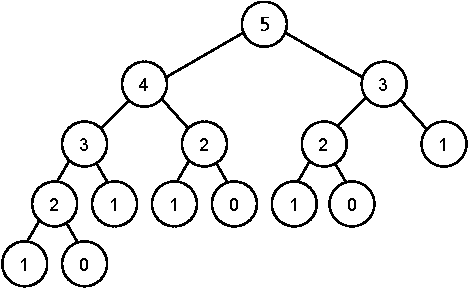
\includegraphics[width=0.7\linewidth, clip]{2-2.pdf}
\end{figure}

図の棒で繋がれている部分は計算に利用することを表しています。\\
図は$F_5$の例ですが、$F_5$を求めるために$F_4$と$F_3$を求める、\\
$F_4$を求めるために$F_3$と$F_2$を…という形になっています。\\
そのため、$F_5$を求めるためには画像の線の部分(関数呼び出し)と$F_5$を求めるための呼び出しを合わせて15回も計算を行う必要があります。
\\ \\ \noindent
このような再帰関数による実装では、数字が1上がるだけで大体2倍の計算量が必要になるため$N$=40でも3億回以上の関数呼び出しが発生してしまいます。\\
最近のパソコンで1秒間に処理できる計算量は$10^9$回程度と言われているので、$N$=43程度で1秒を超えてしまうことになります。
\\ \\ \noindent
そこで注目したいのが図の中の同じ数字の部分で、再帰関数では毎回同じ計算を繰り返していることがわかります。\\
…ところで、同じ計算を効率化するアルゴリズム、ありましたよね。
\\ \\ \noindent
DPの考え方②メモるを使うと、このような場合に大幅な効率化ができるようになります。

\clearpage
\noindent
メモを利用したコードを以下に示します。

\begin{lstlisting}[style = customC]
#include <stdio.h>

/* メモ用配列の宣言 */
int dp[100];

int fib(int n)
{
    /* メモがある場合はメモの値を返す */
    if (dp[n] != -1) return dp[n];

    /* メモがない時は計算結果をメモしながら再帰する */
    return dp[n] = fib(n - 2) + fib(n - 1);
}

int main(void) 
{
    int n;

    /* 入力 */
    scanf("%d", &n);
    /* 入力ここまで */

    /* dp配列を-1で初期化する */
    for (int i = 0; i < 100; i++) dp[i] = -1;

    /* fib(0) = 0, fib(1) = 1*/
    dp[0] = 0;
    dp[1] = 1;

    /* 関数を呼び出して戻り値を出力する */
    printf("%d", fib(n));

    return 0; 
}
\end{lstlisting}

\noindent
一般にこのような方法をメモ化再帰と呼びます。\\
このメモ化再帰、もちろんDPの一種ではありますが前の章で使ったような前から順番に計算していくDPと比較するとメリットとデメリットがあります。
\\ \\ \noindent
まずメリットとして、

\begin{itemize}
    \item 漸化式をそのまま実装できる
\end{itemize}

\noindent
という点があります。これはかなり強力なメリットで、参照の順番等を考えなくても必要な順に勝手に再帰してくれるため雑な実装をする際にはかなり重宝します。
\\ \\ \noindent
デメリットとしては、

\begin{itemize}
    \item 再帰関数を見慣れていないと挙動がわかりづらい
    \item メモリ使用量が多い
    \item 言語によっては再帰上限がある場合がある
\end{itemize}

\noindent
などの点があります。\\
このうち3つ目の再帰上限がかなり厄介で、C言語でもスタックに利用されるメモリ領域を使い切るとスタックオーバーフローが発生してしまいます。
\\ \\ \noindent
そこで、今回はメモ化再帰ではなく、応用の効きやすい前から順に計算していくようなDPについて考えていきます。

\clearpage

\subsubsection{漸化式をプログラミングする}

\noindent
ここで、フィボナッチ数列の漸化式を思い出してほしいんですが、

\begin{itemize}
    \item $F_0 = 0$
    \item $F_1 = 1$
    \item $F_{n+2} = F_{n} + F_{n+1}(n \geq 0)$
\end{itemize}

\noindent
こんな形になっていました。\\
この3つ目の式を少し変形すると、

\begin{itemize}
    \item $F_0 = 0$
    \item $F_1 = 1$
    \item $F_{n} = F_{n-2} + F_{n-1}(n \geq 2)$
\end{itemize}

\noindent
このような形に直すことができます。
\\ \\ \noindent
この形の式であれば、$F_0$と$F_1$があれば$F_2$が求められる、$F_1$と$F_2$があれば$F_3$が求められる、…といったように前から順に求めていくことができそうです。
\\ \\ \noindent
ということで、以上の内容や1章の内容を利用して次の問題を解いてみてください。
\\ \\ \noindent
一応前から計算するDPで解くことを想定していますが、メモ化再帰を利用しても問題ありません。

\clearpage

\subsubsection{フィボナッチ数列}
\noindent
{\LARGE 問題文}\\ \hrulefill \\

\noindent
整数$N$が与えられるので、フィボナッチ数列の$N$番目の数字を出力してください。\\
フィボナッチ数列は以下の式で表される数列です。

\begin{itemize}
    \item $F_0 = 0$
    \item $F_1 = 1$
    \item $F_{n+2} = F_{n} + F_{n+1}(n \geq 0)$
\end{itemize}

\noindent
{\LARGE 制約}\\ \hrulefill \\

\noindent
・$2 \leq N \leq 45$
\\ \\
\noindent
{\LARGE 入力}\\ \hrulefill \\

\noindent
入力は以下の形式で標準入力から与えられる。 

\noindent
$N$
\\ \\
\noindent
{\LARGE 出力}\\ \hrulefill \\

\noindent
1行で、フィボナッチ数列の第$N$項を出力せよ。

\clearpage

\subsubsection{問題の解説}

\noindent
制約の$N\leq45$より、単純な再帰関数では時間内に計算できないためDPを利用して解く必要があります。\\
DPによる実装の場合

\begin{itemize}
    \item $F_0 = 0$
    \item $F_1 = 1$
    \item $F_{n} = F_{n-2} + F_{n-1} (n \geq 2)$
\end{itemize}

\noindent
という形式で実装が行えるためこの通りにプログラムを書けばいいです。
\\ \\ \noindent
具体的には、途中計算結果を保存する配列を用意して$F_2$から$F_N$まで順に計算していくことにより求めることができます。
\\ \\ \noindent
以下に解答例を示します。

\noindent
\begin{lstlisting}[style = customC]
#include <stdio.h>

int main(void) 
{
    /* 入力 */
    int n, dp[50];

    scanf("%d", &n);

    dp[0] = 0;
    dp[1] = 1;

    for (int i = 2; i <= n; i++) {
        dp[i] = dp[i - 2] + dp[i - 1];
    }

    printf("%d", dp[n]);

    return 0;
}
\end{lstlisting}

\clearpage
\noindent
また、今回は推奨していませんがメモ化再帰による実装も可能です。\\
一応、以下に解答例を示します。

\noindent
\begin{lstlisting}[style = customC]
#include <stdio.h>

int dp[50];

int fib(int num)
{
    if (dp[num] >= 0) return dp[num];

    return dp[num] = fib(num - 2) + fib(num - 1);
}

int main(void) 
{
    /* 入力 */
    int n;
    scanf("%d", &n);

    /* dp配列の初期化 */
    for (int i = 0; i < 50; i++){
        dp[i] = -1;
    }
    dp[0] = 0;
    dp[1] = 1;

    printf("%d", fib(n));

    return 0;
}
\end{lstlisting}

\noindent
Java/Python/C++の解答例は以下を確認してください。\\
解答例(Gist)[リンク]

\clearpage

\subsubsection{Gistの解答例}
\noindent
基本的にはC言語と同じように

\begin{itemize}
    \item $F_0 = 0$
    \item $F_1 = 1$
    \item $F_{n} = F_{n-2} + F_{n-1} (n \geq 2)$
\end{itemize}

を実装すればいいです。
\\ \\
\noindent
C++による解答例
\begin{lstlisting}[style = customCpp]
// C++の場合

#include <bits/stdc++.h>
// #include <iostream>

using namespace std;

int main(void) {
    int n, dp[50];
    cin >> n;

    dp[0] = 0;
    dp[1] = 1;

    for (int i = 2; i <= n; i++){
        dp[i] = dp[i - 1] + dp[i - 2];
    }

    cout << dp[n] << endl;
    
    return 0;
}
\end{lstlisting}

\noindent
Javaによる解答例
\begin{lstlisting}[style = customJava]
// Javaの場合

import java.util.*;

public class Main {
    public static void main(String[] args) {
        int n;
        Scanner sc = new Scanner(System.in);
        n = Integer.parseInt(sc.next());

        int dp[] = new int[50];
        dp[1] = 1;

        for (int i = 2; i <= n; i++) {
            dp[i] = dp[i - 1] + dp[i - 2];
        }

        System.out.println(dp[n]);
    }
}
\end{lstlisting}

\clearpage

\noindent
Python3による解答例
\begin{lstlisting}[style = customPy]
# Pythonの場合

n = int(input())

dp = [0] * 50

dp[1] = 1

for i in range(2, n + 1):
    dp[i] = dp[i - 1] + dp[i - 2]
    
print(dp[n])
\end{lstlisting}

\clearpage

\subsubsection{トリボナッチ数列}
\noindent
{\LARGE 問題文}\\ \hrulefill \\

\noindent
整数$N$が与えられるので、トリボナッチ数列の$N$番目の数字を出力してください。\\
トリボナッチ数列は以下の式で表される数列です。

\begin{itemize}
    \item $F_0 = 0$
    \item $F_1 = 0$
    \item $F_2 = 1$
    \item $F_{n+3} = F_{n} + F_{n+1}+ F_{n+2}(n \geq 0)$
\end{itemize}

\noindent
{\LARGE 制約}\\ \hrulefill \\

\noindent
・$2 \leq N \leq 38$
\\ \\
\noindent
{\LARGE 入力}\\ \hrulefill \\

\noindent
入力は以下の形式で標準入力から与えられる。 

\noindent
$N$
\\ \\
\noindent
{\LARGE 出力}\\ \hrulefill \\

\noindent
1行で、トリボナッチ数列の第$N$項を出力せよ。

\clearpage

\subsubsection{問題の解説}

\noindent
フィボナッチ数列と同様にDPを利用して実装することができます。\\
トリボナッチ数列を表す漸化式は

\begin{itemize}
    \item $F_0 = 0$
    \item $F_1 = 0$
    \item $F_2 = 1$
    \item $F_{n+3} = F_{n} + F_{n+1}+ F_{n+2}(n \geq 0)$
\end{itemize}

であることから、フィボナッチ数列と同様に変形を行い

\begin{itemize}
    \item $F_0 = 0$
    \item $F_1 = 0$
    \item $F_2 = 1$
    \item $F_{n} = F_{n - 3} + F_{n-2}+ F_{n-1}(n \geq 3)$
\end{itemize}

\noindent
という形式で実装が行えるためこの通りにプログラムを書けばいいです。
\\ \\ \noindent
以下に解答例を示します。

\noindent
\begin{lstlisting}[style = customC]
#include <stdio.h>

int main(void) 
{
    /* 入力 */
    int n, dp[50];

    scanf("%d", &n);

    dp[0] = 0;
    dp[1] = 0;
    dp[2] = 0;

    for (int i = 3; i <= n; i++) {
        dp[i] = dp[i - 3] + dp[i - 2] + dp[i - 1];
    }

    printf("%d", dp[n]);

    return 0;
}
\end{lstlisting}

\noindent
Java/Python/C++の解答例は以下を確認してください。\\
解答例(Gist)[リンク]

\clearpage

\subsubsection{Gistの解答例}
\noindent
C言語と同様に実装が可能です。
\\ \\
\noindent
C++による解答例
\begin{lstlisting}[style = customCpp]
#include <bits/stdc++.h>
// #include <iostream>

using namespace std;

int main(void) {
    int n, dp[50];
    cin >> n;

    dp[0] = 0;
    dp[1] = 0;
    dp[2] = 1;

    for (int i = 3; i <= n; i++){
        dp[i] = dp[i - 1] + dp[i - 2] + dp[i - 3];
    }

    cout << dp[n] << endl;
    
    return 0;
}
\end{lstlisting}

\noindent
Javaによる解答例
\begin{lstlisting}[style = customJava]
import java.util.*;

public class Main {
    public static void main(String[] args) {
        int n;
        Scanner sc = new Scanner(System.in);
        n = Integer.parseInt(sc.next());

        int dp[] = new int[50];
        dp[2] = 1;

        for (int i = 3; i <= n; i++) {
            dp[i] = dp[i - 1] + dp[i - 2] + dp[i - 3];
        }

        System.out.println(dp[n]);
    }
}
\end{lstlisting}

\noindent
Python3による解答例
\begin{lstlisting}[style = customPy]
n = int(input())

dp = [0] * 50

dp[2] = 1

for i in range(3, n + 1):
    dp[i] = dp[i - 1] + dp[i - 2] + dp[i - 3]
    
print(dp[n])
\end{lstlisting}

\clearpage


\section{C言語版セッションで追加した項目}
\subsection{はじめに}

\noindent
{\LARGE 言語について}\\ 
本教材では、基本的にC言語を利用しています。\\
他言語の利用については以下のようになっています。\\
利用できる言語一覧についてはこちらから確認してください。 \\

\begin{table}[H]
    \centering
    \begin{tabular}{|c||c|c|c|}
        \hline
        言語 & 教材中のコード例 & 解答への利用 & 解答例 \\ \hline
        \hline
        C言語 & 〇 & 〇 & 〇\\ \hline
        \begin{tabular}{c}
            Java\\Python3\\C++
        \end{tabular} & × & 〇(*1) & 〇\\ \hline
        その他言語 & × & 〇(*1) & ×\\ \hline
    \end{tabular}
\end{table}

\noindent
*1:C言語以外を利用するには他言語版セッションに参加する必要があります。
\\ \\ \noindent
{\LARGE 教材中の表現について}\\ 
{\Large 計算量}\\ 
教材中では「計算量」という表現が多く出てきます。\\
これは、厳密には時間計算量と呼ばれるもので答えを出すまでにかかる計算回数を表しています。\\
本教材中での認識としては計算量を減らすとかかる時間が短くなる、程度の認識で問題ありません。\\
より深く知りたい場合は以下のようなキーワードを調べてみるといいかもしれません。

\begin{itemize}
    \item オーダ記法(オーダー記法、O記法) 
    \item ランダウの記号
    \item 時間計算量
\end{itemize}

\clearpage
\noindent
{\LARGE 問題について}\\ 
{\Large 問題の形式}\\ 
本教材で利用する問題は、複数パターンの入力例に対してそれぞれ答えを出力する形式となっています。\\
よって、解答となるプログラムは以下のような流れになっている必要があります。

\begin{enumerate}
    \item 入力を受け取る
    \item 何らかの処理をする(問題により変化する)
    \item 出力を行う
\end{enumerate}

\noindent
サンプルのみを確認して入力値を定数としないように注意してください。
\\ \\ \noindent
{\Large 入出力}\\ 
C言語での入出力一覧は次の教材に纏めてあります。\\
必要に応じて参照してください。
\\ \\ \noindent
{\Large 問題文について}\\ 
問題文は以下の形式になっています。
\\ \\ \noindent
{\LARGE 問題文}\\ \hrulefill \\

\noindent
問題文の本文です。\\
ここにある問題をプログラムを用いて解きます。 
\\ \\ \noindent
{\LARGE 制約}\\ \hrulefill \\

\noindent
入力値の範囲です。\\
$0 \leq N \leq 100$であれば $N$ が0から100の範囲のいずれかを取ることを示しています。 
\\ \\
\noindent
{\LARGE 入力}\\ \hrulefill \\

\noindent
入力の形式です。\\
ここに示される形式で入力値が与えられます。 
\\ \\
\noindent
{\LARGE 出力}\\ \hrulefill \\

\noindent
出力の形式です。\\
ここに示される形式で出力を行う必要があります。 
\\ \\
\noindent
{\LARGE サンプルケース}\\ \hrulefill \\

\noindent
入力のサンプルケースです。\\
実際の採点ではここにあるケースに加え複数のケースで判定を行います。 

\clearpage

\subsection{C言語入出力チートシート}

\noindent
ここでは、C言語における基本的な入出力の方法を確認できます。\\
なお、C言語の標準入力では空白区切り、行区切り共に同じように取得することが可能です。
\\ \\ \noindent
{\LARGE 入力編}\\ \hrulefill \\
{\Large 1つの整数の入力}\\ 
入力\\
$N$
\\ \\ \noindent
$N$は整数

\noindent
\begin{lstlisting}[style = customC]
int n;
scanf("%d", &n);
\end{lstlisting}

\noindent
{\Large 2つの整数の入力}\\ 
入力\\
$N$ $M$
\\ \\ \noindent
$N$, $M$は整数

\noindent
\begin{lstlisting}[style = customC]
int n, m;
scanf("%d", &n);
scanf("%d", &m);
\end{lstlisting}

\noindent
{\Large 整数列の入力}\\ 
入力\\
$N$\\
$A_1, A_2, ..., A_N$
\\ \\ \noindent
$N$, $A_i$は整数\\

\noindent
\begin{lstlisting}[style = customC]
int n, a[101];
scanf("%d", &n);
for(int i = 0; i < n; i++){
    scanf("%d", &a[i]);
}
\end{lstlisting}

\clearpage
\noindent
{\Large 1行1文字の入力}\\ 
入力\\
$C$
\\ \\ \noindent
$C$は半角文字\\

\noindent
\begin{lstlisting}[style = customC]
char c;
scanf("%c", &c);
\end{lstlisting}

\noindent
{\Large 1行の文字列の入力}\\ 
入力\\
$S$
\\ \\ \noindent
$S$は文字列\\

\noindent
\begin{lstlisting}[style = customC]
char s[101];
scanf("%s", s);
\end{lstlisting}

\noindent
{\LARGE 出力編}\\ \hrulefill \\
{\Large 1つの整数の出力}\\ 
出力\\
$N$\\
\\ \\ \noindent
$N$は整数

\noindent
\begin{lstlisting}[style = customC]
int n;
printf("%d\n", n);
\end{lstlisting}

\noindent
{\Large 整数列の出力(行区切り)}\\ 
出力\\
$A_1$\\
$A_2$\\
$:$\\
$A_N$
\\ \\ \noindent
$N$, $A_i$は整数

\noindent
\begin{lstlisting}[style = customC]
int n, a[101];
for(int i = 0; i < n; i++){
    printf("%d\n", a[i]);
}
\end{lstlisting}

\noindent
{\Large 整数列の出力(空白区切り)}\\ 
出力\\
$A_1$ $A_2$ $...$ $A_N$
\\ \\ \noindent
$N$, $A_i$は整数

\noindent
\begin{lstlisting}[style = customC]
int n, a[101];
for(int i = 0; i < n; i++){
    if(i != 0) putchar(' ');
    printf("%d", a[i]);
}
printf("\n");
\end{lstlisting}

\noindent
{\Large 1行の文字列の出力}\\ 
入力\\
$S$
\\ \\ \noindent
$S$は文字列

\noindent
\begin{lstlisting}[style = customC]
char s[101];
printf("%s\n", s);
\end{lstlisting}

\noindent
{\LARGE オマケ}\\ \hrulefill \\
{\Large 十分に大きい数 / 小さい数}\\ 
C言語で大きい数や小さい数を使う場合、シフト演算子を利用して数値を代入することが多いです。\\
シフト演算子はbit表記(2進数)の状態で桁をシフトする演算で、bigの場合は10(2)を左に29ビット算術シフトした値=1073741824となります。\\
これで足りない場合にはlimit.hをincludeすればINT\_MAXにより2147483647が取得できますが…そこまで必要になることはあまりないと思います。\\

\noindent
\begin{lstlisting}[style = customC]
int big = 2 << 29;
int small = -2 << 30;
\end{lstlisting}

\clearpage

\subsection{大きい数 初期プログラム}

\begin{lstlisting}[style = customC]
/* CやC++などシェルに実行結果コード返却を明示する言語を利用する場合 基本的に0を返却してください。 */
#include <stdio.h>

int main(void)
{
    /* 入力 */
    int x, y;
    scanf("%d %d", &x, &y);


    return 0;
}
\end{lstlisting}

\subsection{最大の数 初期プログラム}

\begin{lstlisting}[style = customC]
/* CやC++などシェルに実行結果コード返却を明示する言語を利用する場合 基本的に0を返却してください。 */
#include <stdio.h>

int main()
{
    /* 入力 */
    int n, a[100000];
    scanf("%d", &n);

    for(int i = 0; i < n; i++){
        scanf("%d", &a[i]);
    }


    return 0;
}
\end{lstlisting}

\clearpage

\subsection{フィボナッチ数列 初期プログラム}

\begin{lstlisting}[style = customC]
/* CやC++などシェルに実行結果コード返却を明示する言語を利用する場合 基本的に0を返却してください。 */
#include <stdio.h>

int main(void) 
{
    /* 入力 */
    int n;
    scanf("%d", &n);


    return 0; 
}
\end{lstlisting}

\subsection{トリボナッチ数列 初期プログラム}

\begin{lstlisting}[style = customC]
/* CやC++などシェルに実行結果コード返却を明示する言語を利用する場合 基本的に0を返却してください。 */
#include <stdio.h>

int main(void) 
{
    /* 入力 */
    int n;
    scanf("%d", &n);


    return 0; 
}
\end{lstlisting}

\clearpage

\subsection{さいごに}

\noindent
DPがどんな時に使えるのか、何となく理解できたでしょうか。
\\ \\ \noindent
今回紹介した例は少ないですが、DPが利用できる計算にはこれ以外にも様々なパターンがあります。\\
有名なものだとナップザック問題と呼ばれるものや巡回セールスマン問題(厳密解を求めるもので、要素数が多いと計算できません)などもDPを利用して解くことが可能です。\\
また、BFS(幅優先探索)やDFS(深さ優先探索)、ダイクストラ法(グラフ上の最短経路を求めるアルゴリズム)などもDPを利用した手法だったりします。\\
興味があれば是非色々と調べてみてください。
\\ \\ \noindent
オマケとして、DPに限らず様々なアルゴリズムを学習できるコンテンツを紹介したいと思います。
\\ \\ \noindent
{\Large 超初心者向け}\\
AtCoder Programming Guide for beginners (APG4b)\\
競技プログラミングサイトAtCoderのC++初心者向け講座です。\\
C言語とかめんどくさくて使ってられないけど他の言語の文法とかわからん!という人やC++に興味があるけどなにで勉強すればいいのかわからない、という人におすすめです。
\\ \\ \noindent
{\Large 初心者向け}\\
アルゴ式\\
様々なアルゴリズムが基礎から学べるサイトです。\\
レベル的にはプログラミングの文法はわかるけどアルゴリズムはわからない人向けです。
\\ \\ \noindent
{\Large 中級者向け}\\
Educational DP Contest\\
名前の通りDPを使う問題が沢山載っています。\\
難易度的には比較的簡単に解ける問題(A問題など)から全くもって初心者向けではない問題(J問題以降)など様々な難易度・ジャンルのDP問題があります。
\\ \\ \noindent
Project Euler\\
ガチ勢向け数学コンテストです。\\
英語のみのサイトのため参加のハードルは高めですが英語に慣れていれば良質な問題が多いためオススメです。
\\ \\ \noindent
AtCoder\\
いわゆる競技プログラミングと呼ばれるもののコンテストサイトです。\\
ほぼ毎週コンテストが行われており、DPを利用した問題もたくさん出ています。\\
興味があれば過去問を解いてみるといいかもしれません。
\\ \\ \noindent
TechFUL\\
一応ね、一応同じプラットフォームなので紹介だけ。
色々な問題を解くことができますが採点システムや諸々の導線に若干の難があるので個人的な評価は低め。問題文がわかりづらい。\\
一応コードを書いてると就活に使えたりします。
\\ \\ \noindent
paiza スキルチェック\\
こちらも同様に色々な問題がありますがどんなアルゴリズムを使うかや解答例は非公開なので難易度は高め
コードを書いてると就活に使えたりします。ランクが高いと面接の交通費支給があったりと便利です。
\\ \\ \noindent
その他にも、興味があれば競技プログラミングなどを調べてみると面白いかもしれません。\\
AtCoderなどでは同じ大学の人と競い合ったりもできます。興味があれば、是非。
\\ \\ \noindent
また、オススメの本は以下の通りです。\\
どちらも大学図書館の書架にあるため気になったら是非借りてみてください。

\begin{itemize}
    \item 問題解決力を鍛える!アルゴリズムとデータ構造(大槻兼資)
    \item プログラミングコンテストチャレンジブック(秋葉拓哉)
\end{itemize}

\clearpage

\section{TechFULで教材を表示した場合の例}

\subsection{セクションを利用した際のイメージ}
\begin{figure}[H]
    \centering
    
\includegraphics[width=0.95\linewidth, clip]{techful1.pdf}
\end{figure}


\subsection{教材と問題のイメージ}

\begin{figure}[H]
    \centering
    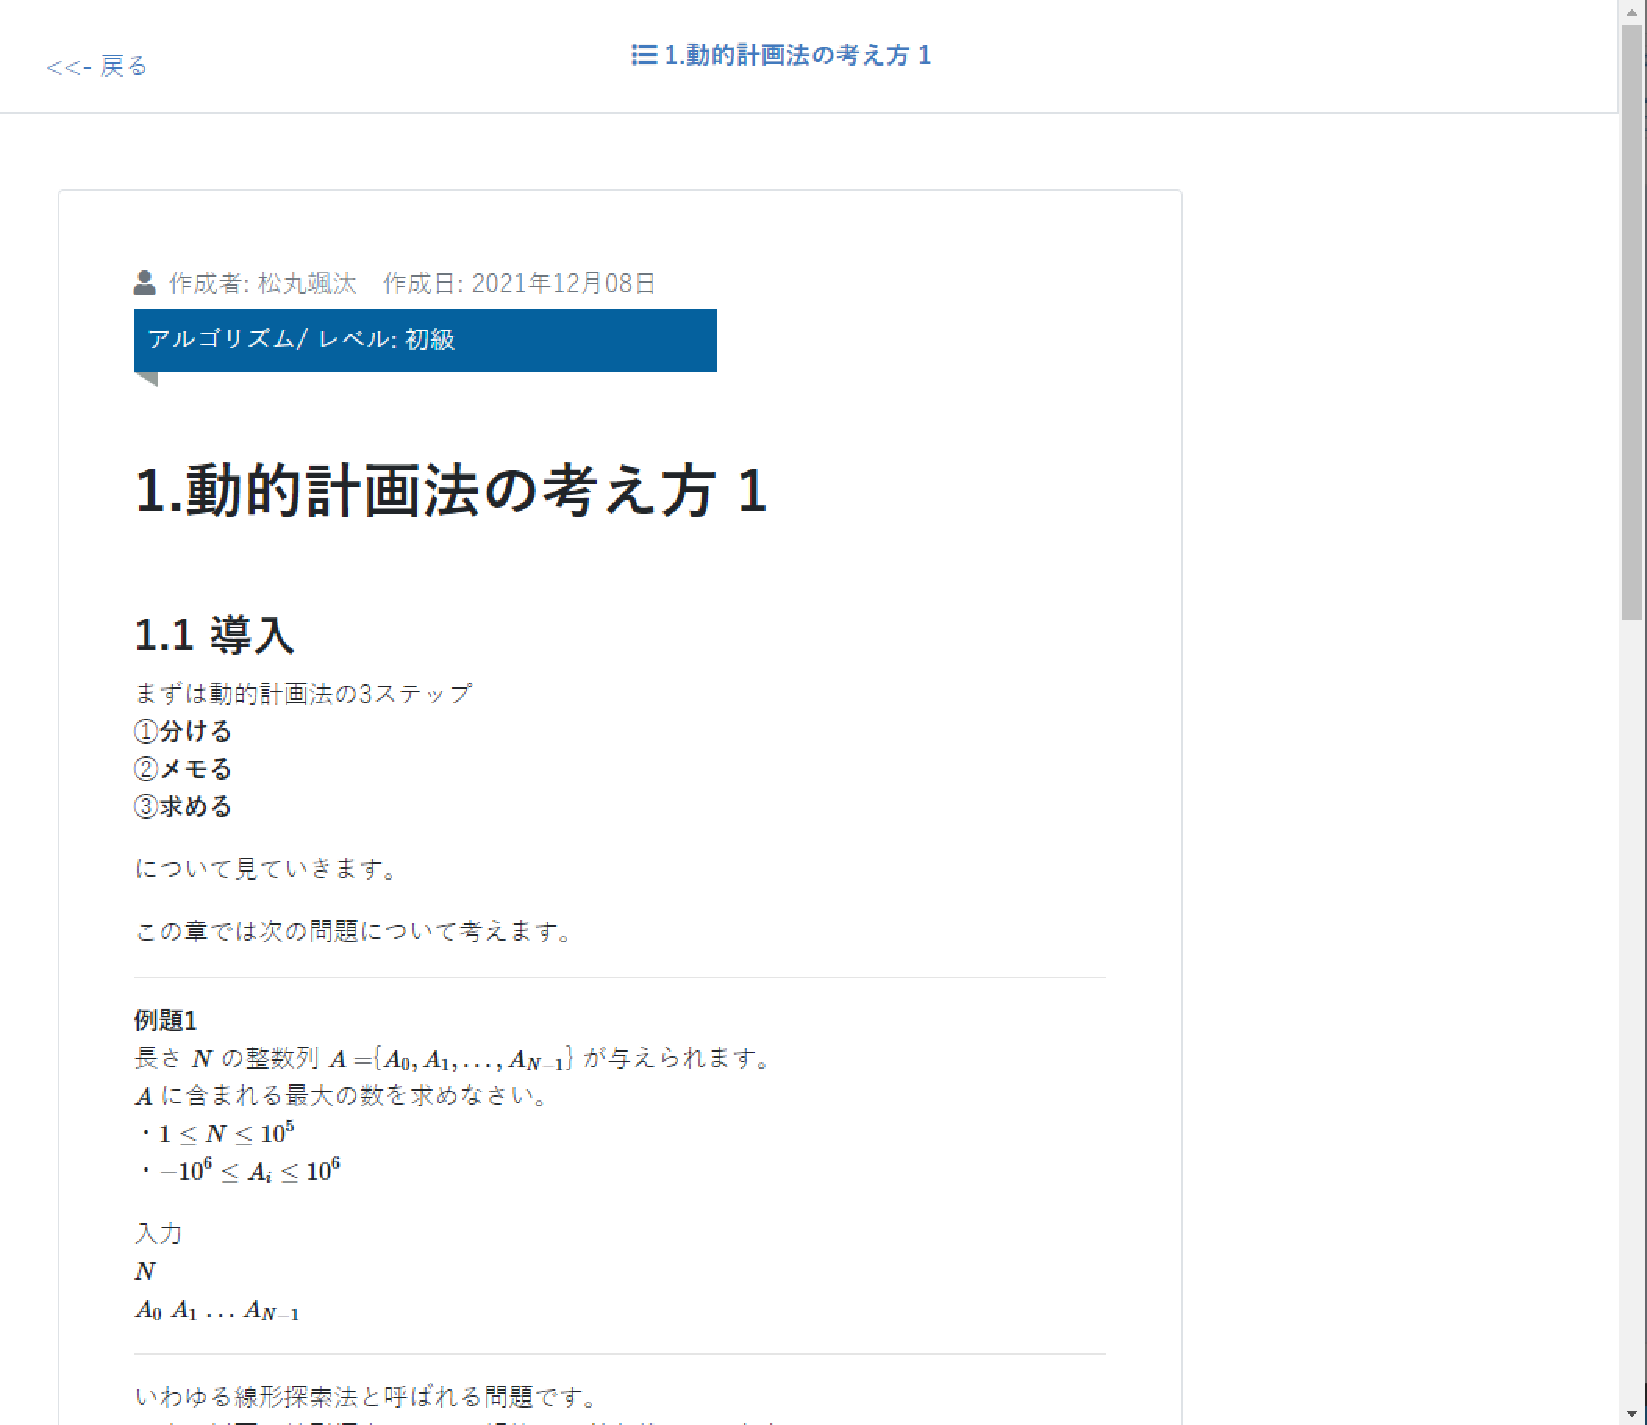
\includegraphics[width=0.95\linewidth, clip]{techful2.pdf}
\end{figure}
\begin{figure}[H]
    \centering
    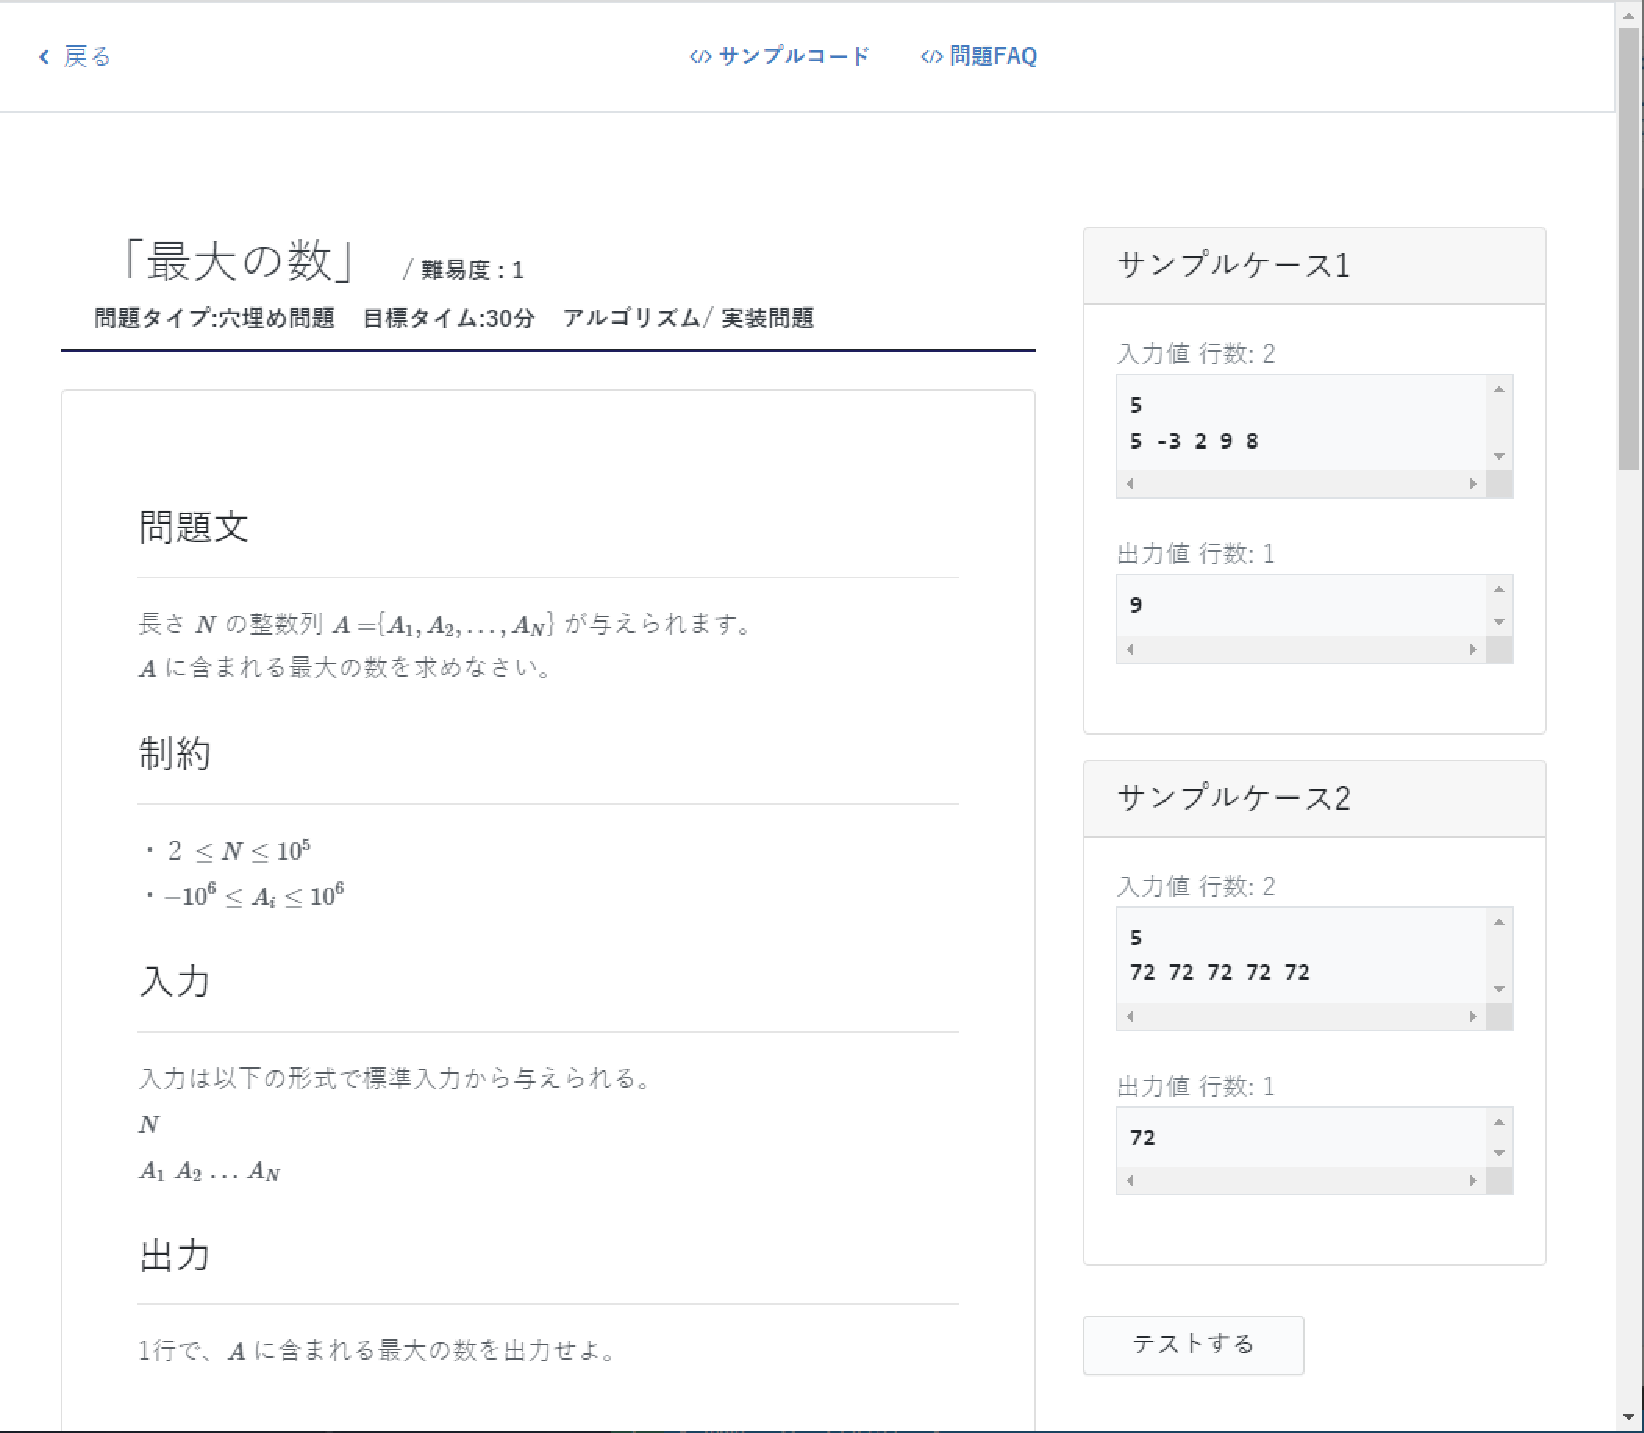
\includegraphics[width=0.95\linewidth, clip]{techful4.pdf}
\end{figure}

\subsection{コードテストを行った時のイメージ}

\begin{figure}[H]
    \centering
    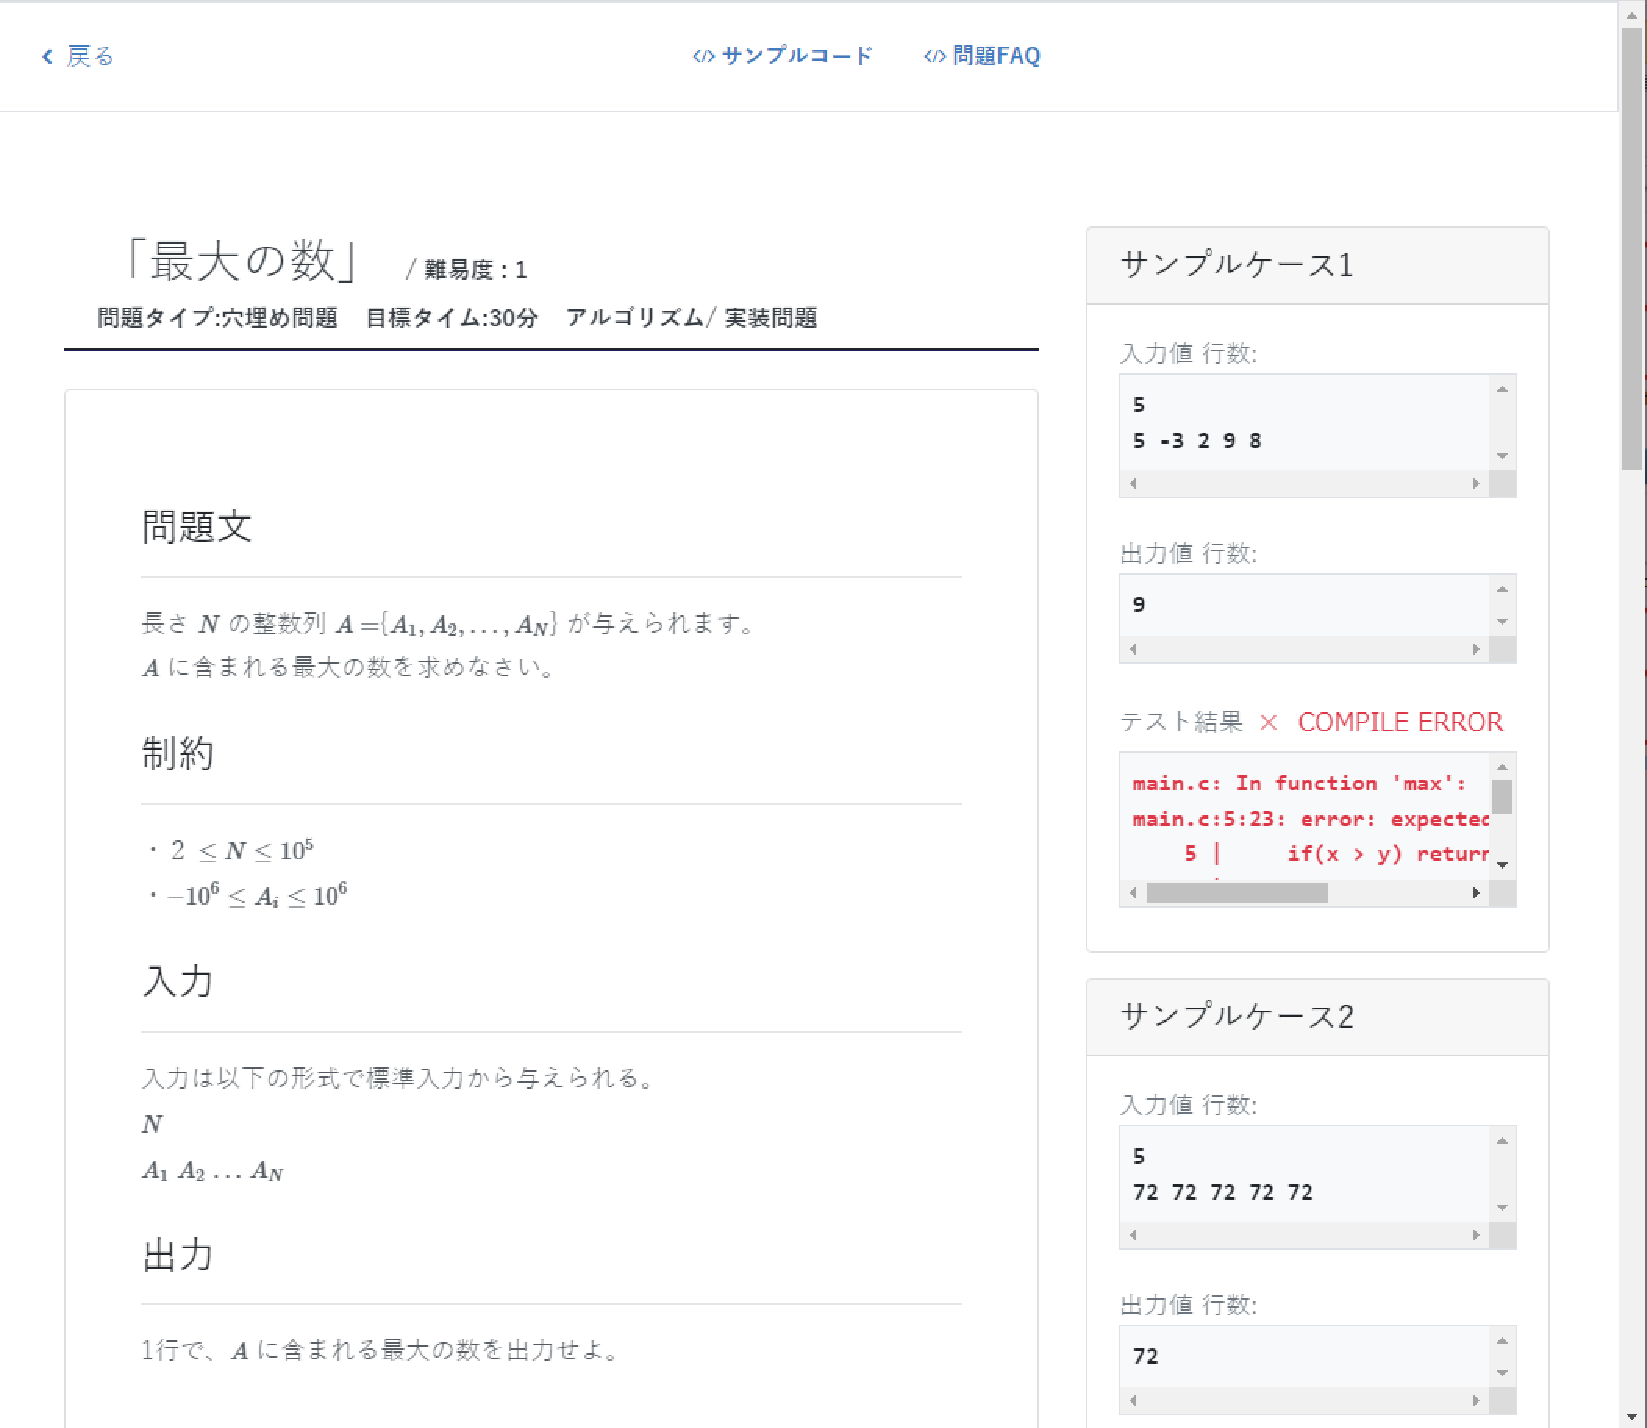
\includegraphics[width=0.95\linewidth, clip]{techful5.pdf}
\end{figure}
\begin{figure}[H]
    \centering
    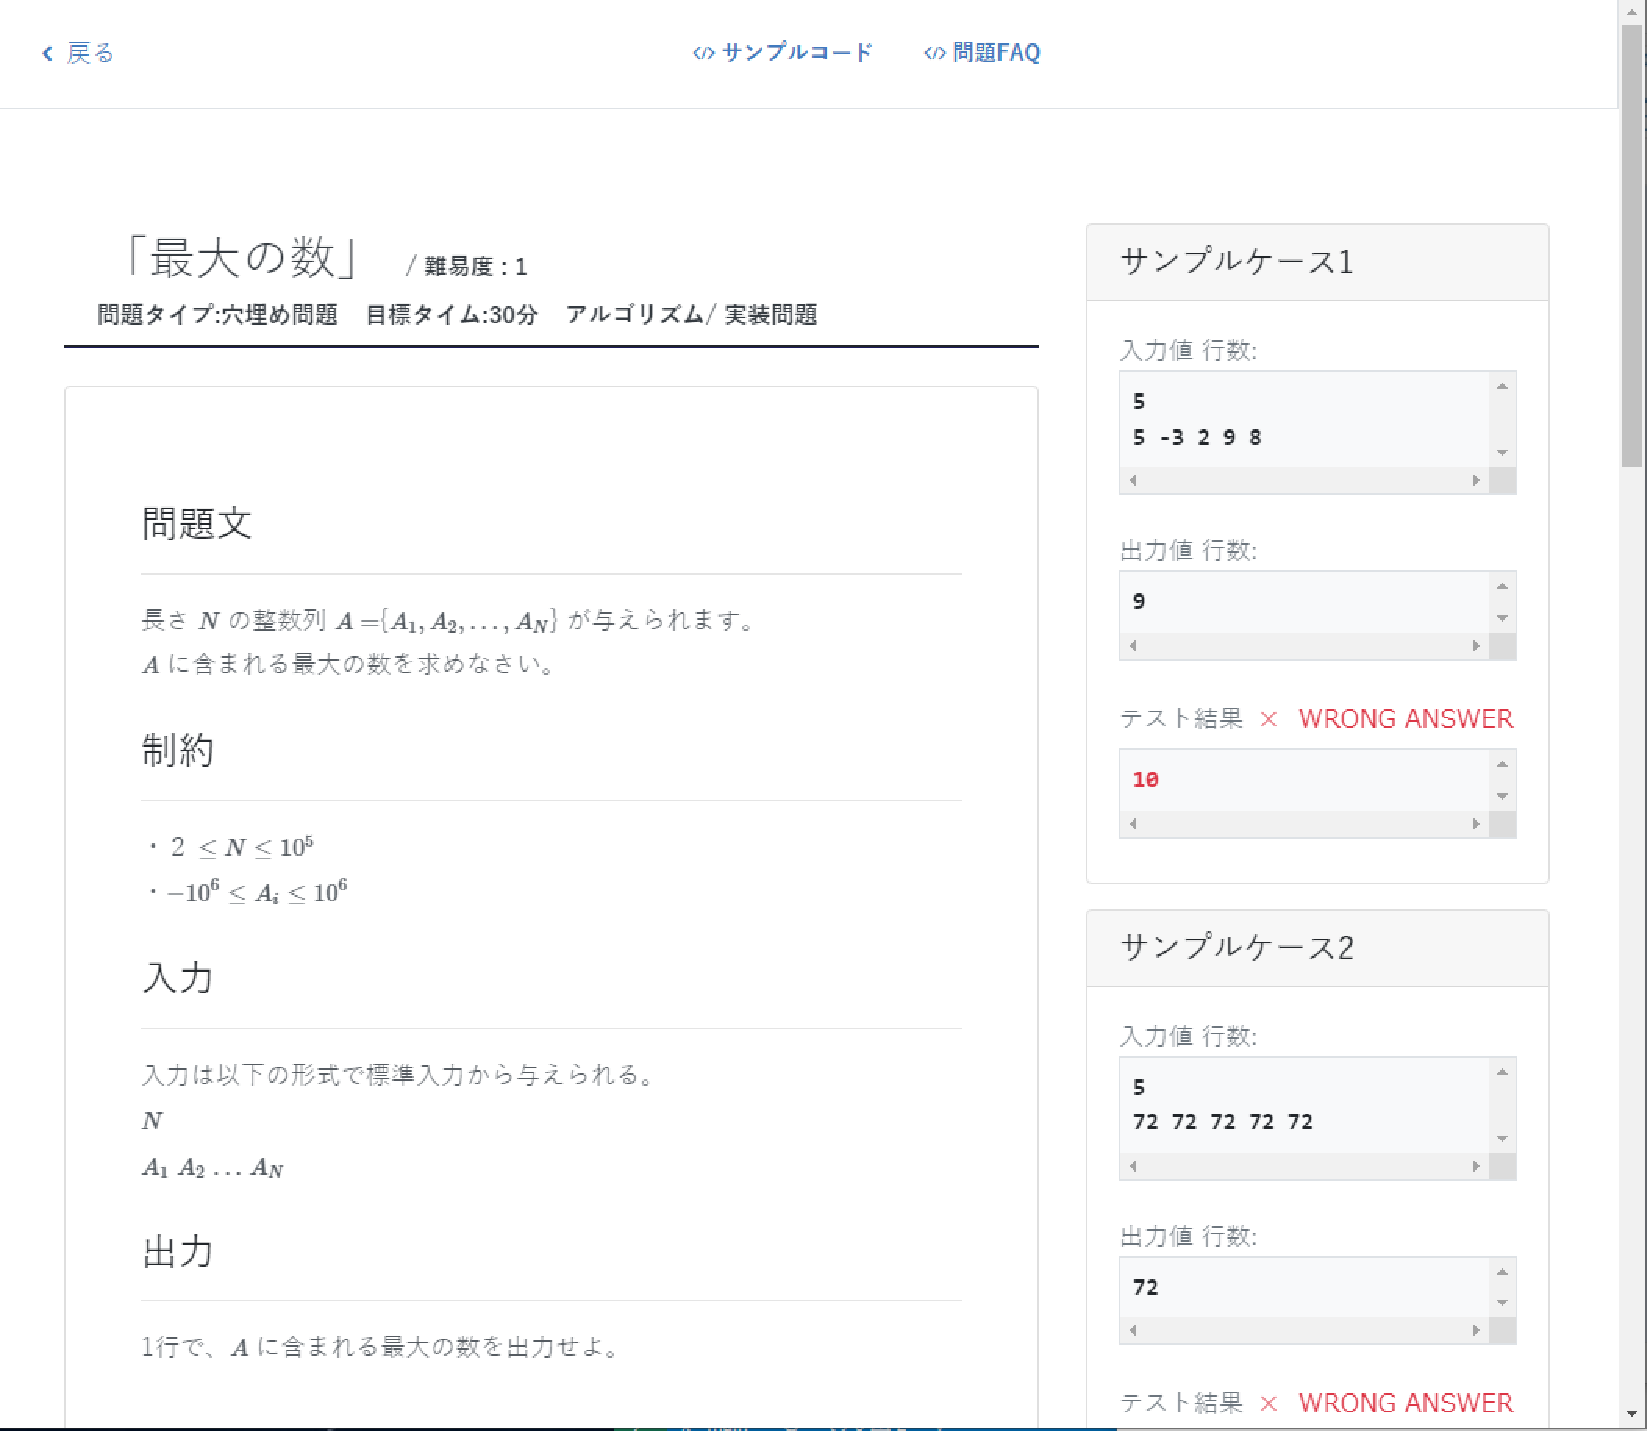
\includegraphics[width=0.95\linewidth, clip]{techful6.pdf}
\end{figure}
\begin{figure}[H]
    \centering
    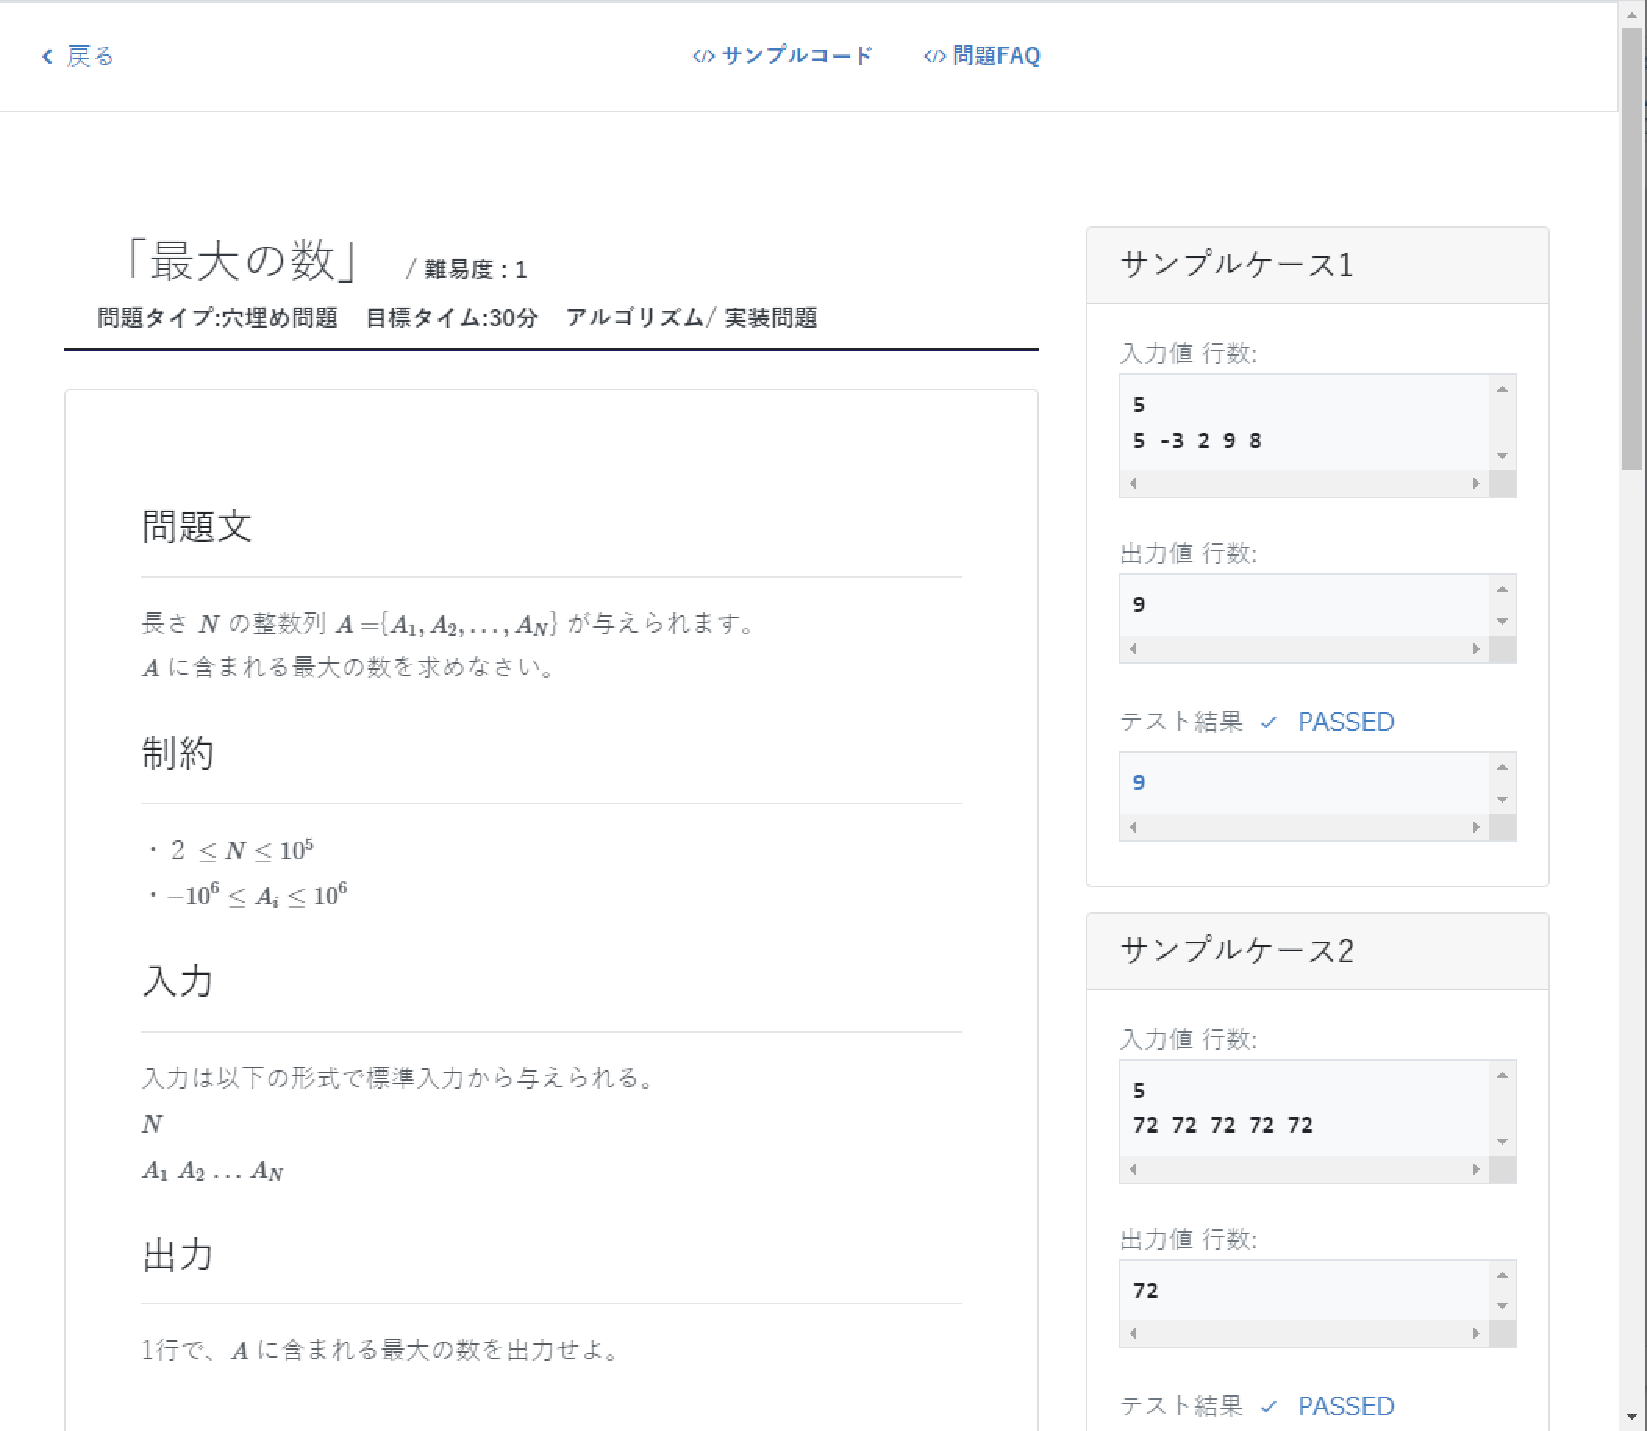
\includegraphics[width=0.95\linewidth, clip]{techful7.pdf}
\end{figure}

\subsection{正誤判定を行った際のイメージ}
\begin{figure}[H]
    \centering
    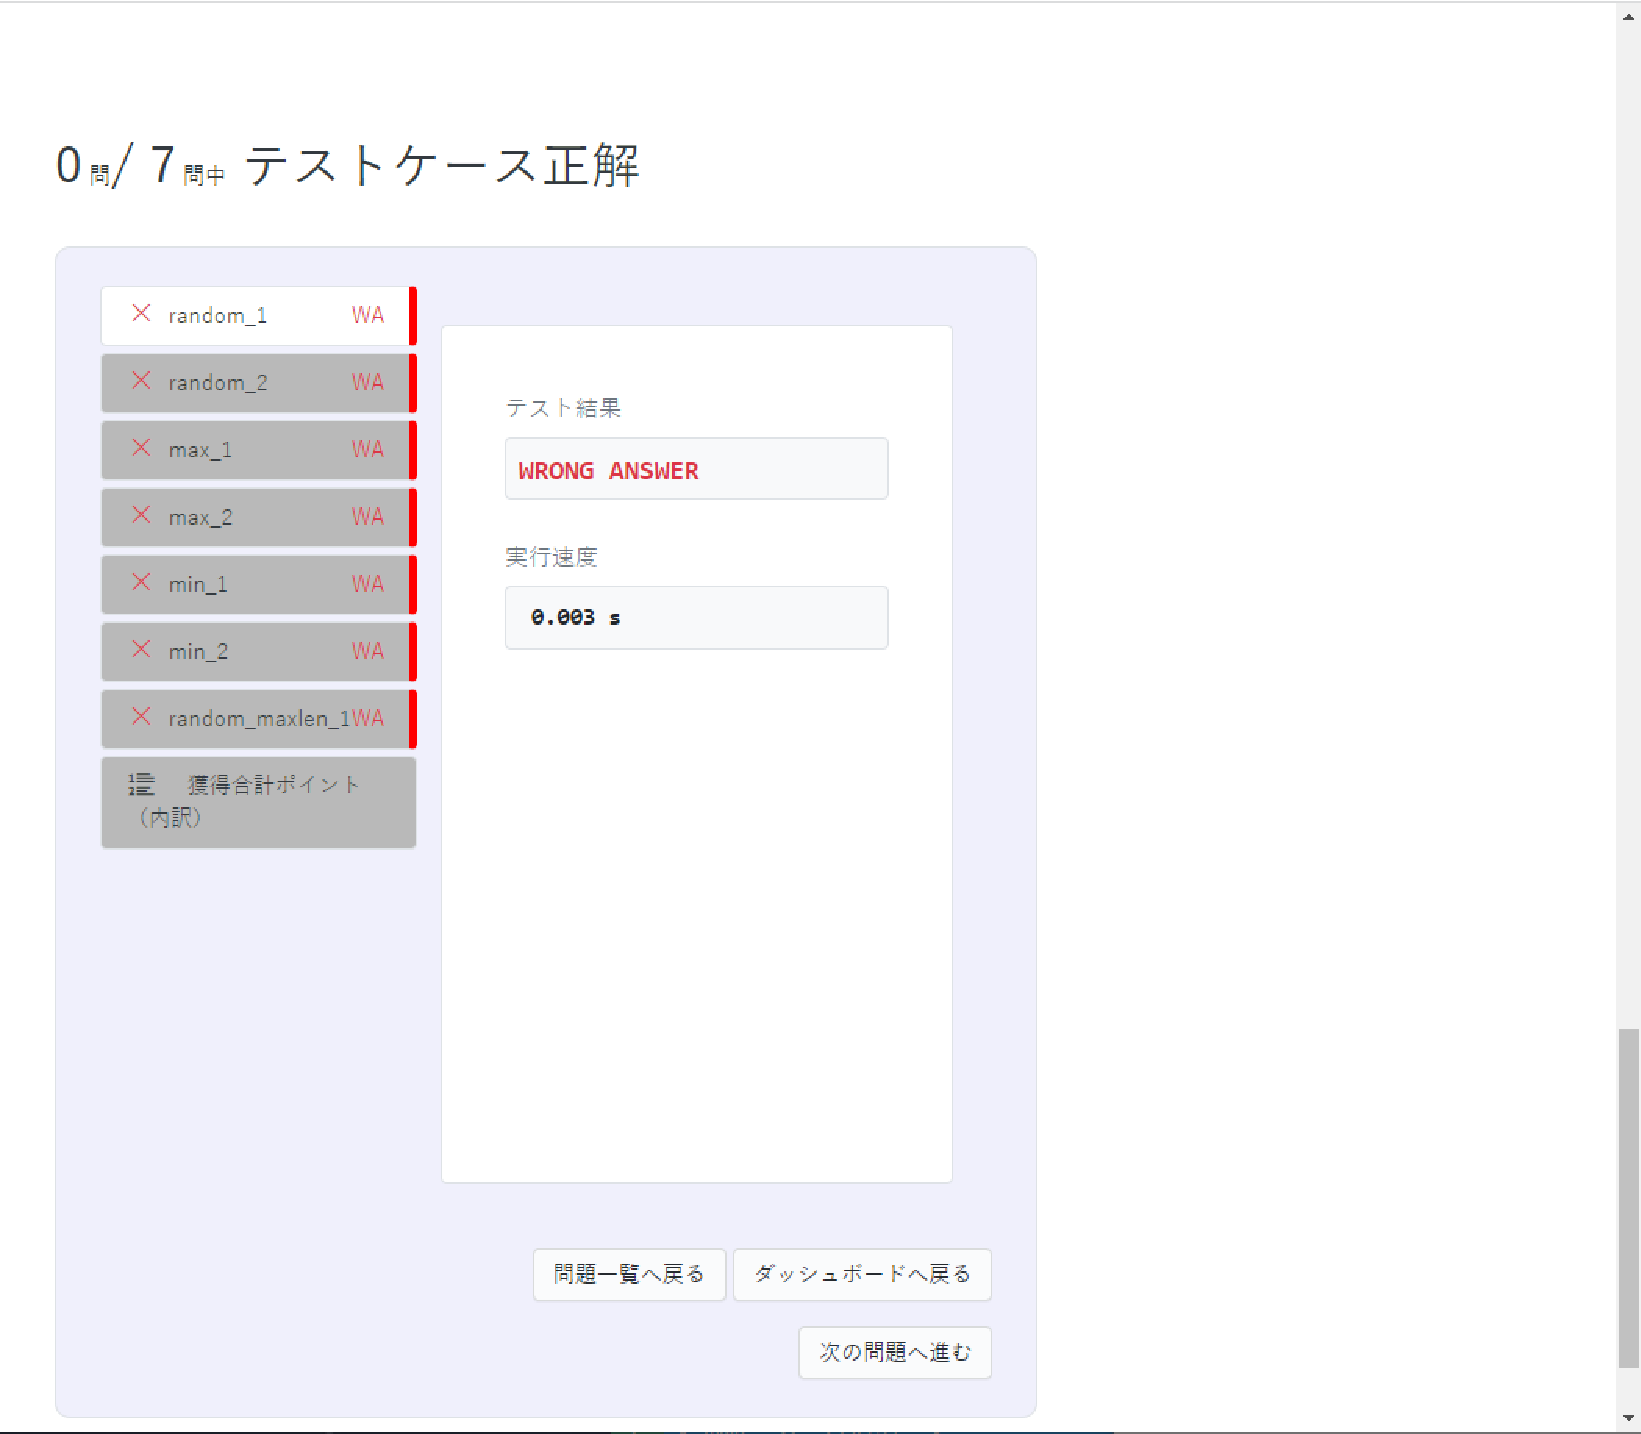
\includegraphics[width=0.95\linewidth, clip]{techful8.pdf}
\end{figure}
\begin{figure}[H]
    \centering
    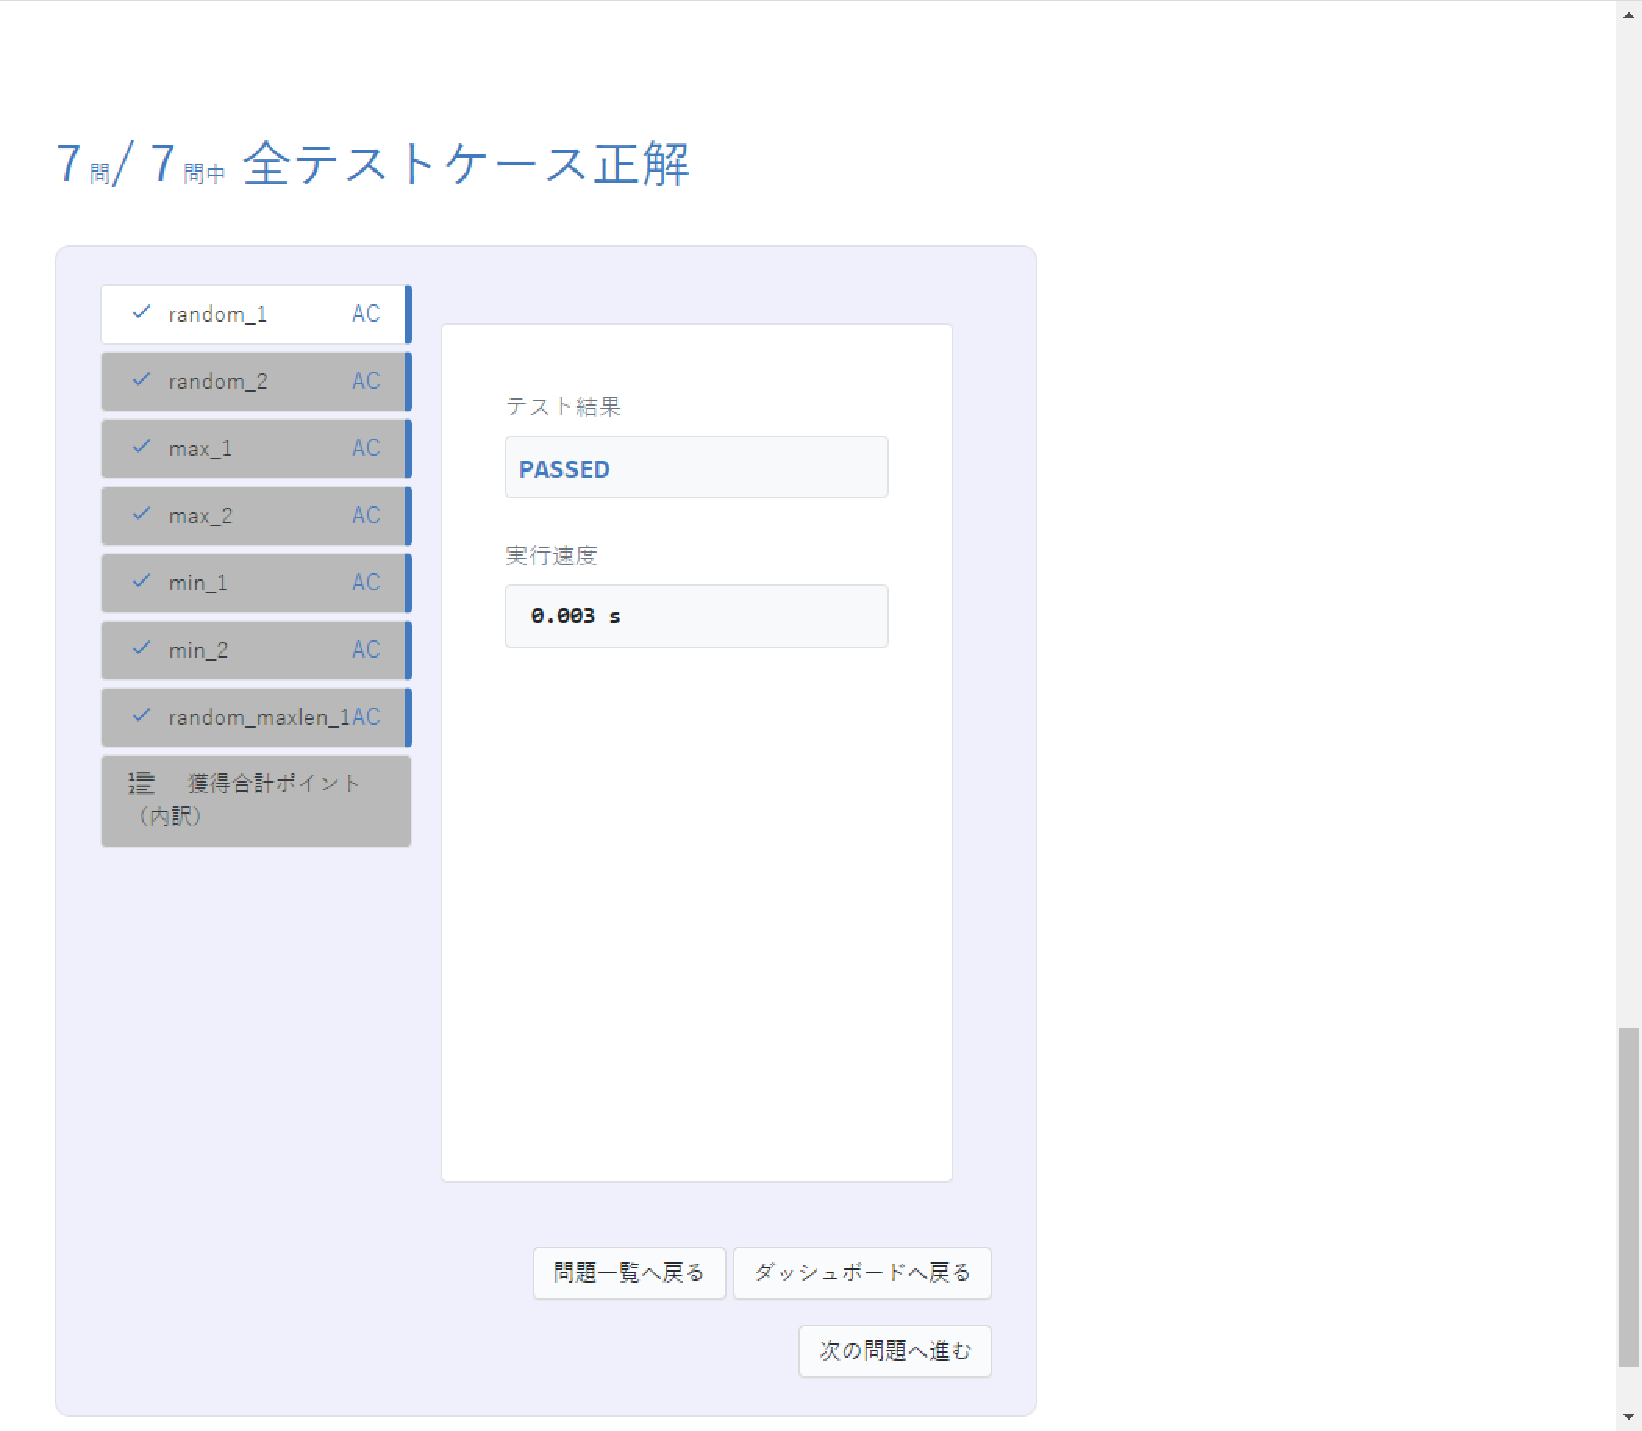
\includegraphics[width=0.95\linewidth, clip]{techful9.pdf}
\end{figure}
